% STEP 1: Choose oneside or twoside. Use the 'draft' option a lot when writing.
\documentclass[english, oneside]{HYgradu}

\usepackage[utf8]{inputenc} % For UTF8 support. Use UTF8 when saving your file.
\usepackage{lmodern} % Font package
\usepackage{textcomp}
\usepackage[pdftex]{color, graphicx} % For pdf output and jpg/png graphics
\usepackage[pdftex, plainpages=false]{hyperref} % For hyperlinks and pdf metadata
\usepackage{fancyhdr} % For nicer page headers
%\usepackage{tikz} % For making vector graphics (hard to learn but powerful)
%\usepackage{wrapfig} % For nice text-wrapping figures (use at own discretion)
\usepackage{amsmath, amssymb} % For better math
\usepackage[sort,colon]{natbib} % For bibliography
\usepackage[footnotesize,bf]{caption} % For more control over figure captions

\fussy % Probably not needed but you never know...

% OPTIONAL STEP: Set up properties and metadata for the pdf file that pdfLaTeX makes.
% But you don't really need to do this unless you want to.
\hypersetup{
    bookmarks=true,         % show bookmarks bar first?
    unicode=true,           % to show non-Latin characters in Acrobat’s bookmarks
    pdftoolbar=true,        % show Acrobat’s toolbar?
    pdfmenubar=true,        % show Acrobat’s menu?
    pdffitwindow=false,     % window fit to page when opened
    pdfstartview={FitH},    % fits the width of the page to the window
    pdftitle={},            % title
    pdfauthor={},           % author
    pdfsubject={},          % subject of the document
    pdfcreator={},          % creator of the document
    pdfproducer={pdfLaTeX}, % producer of the document
    pdfkeywords={something} {something else}, % list of keywords for
    pdfnewwindow=true,      % links in new window
    colorlinks=true,        % false: boxed links; true: colored links
    linkcolor=black,        % color of internal links
    citecolor=black,        % color of links to bibliography
    filecolor=magenta,      % color of file links
    urlcolor=cyan           % color of external links
}

% STEP 2:
% Set up all the information for the title page and the abstract form.
% Replace parameters with your information.
\title{Simulating the dynamics of supermassive black holes}
\author{Vili Oja}
\date{\today}
\level{Master's thesis}
\faculty{Faculty of Science}
\department{Department of Physics}
\address{PL 64 (Gustaf Hällströmin katu 2)\\00014 Helsingin yliopisto\\Finland}
\subject{Astronomy}
\prof{Professor Peter Johansson}
\censors{Professor Peter Johansson}{}{}
\depositeplace{}
\additionalinformation{}
\numberofpagesinformation{\numberofpages \ pages}
\classification{}
\keywords{Your keywords here}
\quoting{}

\begin{document}
\setlength{\parindent}{1cm}
\setlength{\parskip}{0cm}
% Generate title page.
\maketitle

% STEP 3:
% Write your abstract (of course you really do this last).
% You can make several abstract pages (if you want it in different languages),
% but you should also then redefine some of the above parameters in the proper
% language as well, in between the abstract definitions.
\begin{abstract}
Abstract goes here.
\end{abstract}

% Place ToC
\mytableofcontents



% -----------------------------------------------------------------------------------
% STEP 4: Write the thesis.
% Your actual text starts here. You shouldn't mess with the code above the line except
% to change the parameters. Removing the abstract and ToC commands will mess up stuff.
\setlength{\parindent}{.75cm}
\setlength{\parskip}{.6cm}
\chapter{Introduction}


\section{Discovery of black holes}

\section{History of black hole observations}
%miten eri aukkoja havaitaan, binääreissä pieniä aukkoja, keskustoissa suuria ja voidaan nähdä niiden vaikutus ympäröiviin tähtiin

\section{Aim of this thesis}

\chapter{Dynamical modelling of black holes}

\section{Black hole properties}

A black hole (BH) is defined as a region of spacetime for which the gravitational field is so strong that no objects or signals that carry information can escape from it. Black holes have the interesting property that their gravitational field is completely determined by the black hole's mass M, its angular momentum J, and its electric charge Q. This is known as the black hole uniqueness theorem or no-hair theorem, which states that all physical black hole solutions are completely characterized by the above-mentioned three parameters, and must satisfy the condition 
\begin{equation} \label{equ:bhunique}
M^2 - \left( \frac{J}{M} \right)^2 - Q^2 \geq 0 \ ,
\end{equation}
where it's set that $G = c = 1$ \citep{mazur:2001}.
Thus only by changing these variables can the properties of the black hole change. The physical reasoning for this uniqueness theorem is that the matter beyond the event horizon of a black hole cannot directly affect anything outside of it. Thus only the globally conserved characteristics, such as mass and angular momentum, survive and can be detected from the outside. The electric charge of black holes that appear in nature is most likely neutral, since having a non-neutral charge would require vastly different amounts of protons and electrons to enter the black hole, which is not a realistic scenario with normal matter.

Black holes can be divided into four distinct types based on these properties. Every black hole has mass, but the angular momentum and electric charge are not necessary.
\begin{table}[htb]
\centering
\caption{Different types of black holes}
\begin{tabular}{|c|c|c|}
\hline
 & Non-rotating ($J = 0$) & Rotating ($J \neq 0$) \\ \hline
Uncharged ($Q = 0$) & Schwarzschild & Kerr \\ \hline
Charged ($Q \neq 0$) & Reissner–Nordström & Kerr–Newman \\ \hline
\end{tabular}
\end{table}

The simplest type of black hole is created when an object of mass M becomes smaller than the radius
\begin{equation}
r_S = \frac{2GM}{c^2} \ .
\end{equation}
This can happen in nature when a star dies and explodes in a supernova. The core of the star can compress enough to pass the radius and form a black hole. The radius is called the Schwarzschild radius, so named after the German astronomer Karl Schwarzschild, who found an exact solution for the Einstein field equations. The surface at this radius is called the event horizon. Event horizons are mathematical surfaces, and they do not form any sort of physical barrier. An observer can fall inside the event horizon without any problem. The event horizon simply marks the limit at which not even light can escape the gravitational pull of the black hole.

There exists solutions that do not satisfy the condition given by equation \ref{equ:bhunique}, but those are not stationary. A stationary field is one that is in a steady state, but the masses causing that field may be non-static, rotating for instance. So these non-stationary solutions are not in a steady state. This gives an upper limit to the angular momentum that a physical uncharged black hole can have. This limit can be expressed as the specific angular momentum 
\begin{equation} \label{equ:angularmomentum}
a = \frac{J}{Mc}
\end{equation}
or as the dimensionless spin parameter
\begin{equation}
a_* = \frac{Jc}{GM^2} \ .
\end{equation}
The parameter can range from 0, meaning that the hole doesn't spin, to 1, meaning that it spins as fast as possible for a given mass \citep{middleton:2016}.

If a black hole would have even larger angular momentum than allowed by these constraints, it would mean that it actually would not be a black hole at all, since the event horizon would disappear due to the extreme rotation. This is made clear by looking at equation \ref{equ:evenhorizons}, which describes the surfaces that event horizons occur at. If $\mu^2 < a^2$, the solutions for this equation are complex, which is said to mean that the actual event horizons disappear. This would cause what is known as a naked singularity, meaning that a singularity that is normally contained within a black hole would be visible to an outside observer. The possible existence of such singularities in nature is uncertain but extremely unlikely. If they were to exist, they might cause fundamental problems for physics as we know it. We would be able to see matter condensed to infinite density, and we have no theories that can predict how spacetime works near such abnormalities. Normally this is not a problem, since they cannot be observed inside event horizons. However the cosmic censorship hypothesis suggests that naked singularities cannot be formed in nature from realistic initial conditions, which would avoid the problem altogether \citep{wald:1997}. An extremely rapid spin could prevent the collapse into a black hole thanks to the centrifugal forces. The object would have to lose enough of its angular momentum before it could collapse.

Astrophysical black holes that appear in nature are assumed to be most likely Kerr black holes. The normal matter that creates and feeds black holes contains roughly equal amounts of protons and electrons, so the overall electric charge is mostly neutral. But stars do spin around themselves, thus possessing angular momentum. Because of the conservation of angular momentum, the stellar remnant will spin around itself as well. And even black holes with small amounts of angular momentum can gain more of it through its interactions with surrounding matter. Infalling matter creates an accretion disk around the hole. The matter in the inner parts of the accretion disk loses angular momentum and moves inwards due to friction, causing angular momentum to move outwards in the disk. Eventually the matter will fall within the event horizon, conferring its mass and remaining angular momentum to the black hole, speeding up its rotation \citep{bhphysics}. Black holes are also capable of losing their angular momentum. One way for this to happen is through the emission of jets.

\subsection{The structure of a rotating black hole}

While Schwarzschild black holes have only the one event horizon and a point-like singularity in the middle, spinning black holes are far more complicated. All massive objects cause what is known as the geodetic effect, or de Sitter precession. This is predicted by general relativity, and causes orbiting bodies to precess due to the effects of gravity. In addition to this, spinning sources of gravity cause an additional effect called Lense-Thirring precession or frame-dragging. The massive object drags the surrounding spacetime with it as it spins, causing nearby particles and photons to rotate too, even if they did not have any angular momentum of their own to begin with. This effect is significant only around very massive objects, like black holes. At certain point this effect becomes so strong that any object, including light, \textit{must} spin along the rotation of the black hole. It's impossible for them to stay still. This limit is known as the stationary limit surface, and it is described in the equation \ref{equ:statlimsurf}. The area inside this limit is called the ergosphere, so named after the Greek word for work. The ergosphere differs from the insides of an event horizon because particles that fall into it can actually still escape from this region. If a particle escapes from the ergosphere, it converts some of the black hole's rotation energy into it's own momentum \citep{grintro}. This lowers the angular momentum of the black hole, and the process could theoretically over time cause a rotating black hole to spin lower and lower.

%This is called the Penrose process, and it is a possible explanation for some highly energetic astrophysical phenomena, such as gamma ray bursts. 
%TODO tarkenna tätä kappaletta

The Kerr metric is often presented in Boyer-Lindquist coordinates $(t, r, \theta, \phi)$ which are similar to spherical polar coordinates and are related to Cartesian coordinates via the following transforms:
\begin{align*}
x &= \sqrt{r^2 + a^2} \mathrm{sin}\theta \mathrm{cos}\phi \\
y &= \sqrt{r^2 + a^2} \mathrm{sin}\theta \mathrm{sin}\phi \\
z &= r \mathrm{cos}\theta
\end{align*}
The variable $a$ is the same specific angular momentum as in the equation \ref{equ:angularmomentum}. The only true singularity (i.e. a singularity that exists no matter what coordinate system we choose) in the Kerr metric occurs when $r=0$ and $\theta = \pi/2$ \citep{grintro}. It's easy to see that in Cartesian coordinates this corresponds to a flat ring in the equatorial plane with the radius of $a$. So rotating black holes don't have a point singularity, but a ring singularity instead.

In addition there exists coordinate singularities (i.e. singularities we can get rid of if we choose our coordinates differently) as well. These singularities occur on the surfaces
\begin{equation} \label{equ:evenhorizons}
r_\pm = \mu \pm (\mu^2 - a^2)^{1/2}
\end{equation}
which describe the event horizons of the black hole, and on the surfaces
\begin{equation} \label{equ:statlimsurf}
r_{S \pm} = \mu \pm (\mu^2 - a^2 \mathrm{cos}^2 \theta)^{1/2}
\end{equation}
which describe the stationary limit surfaces of the black hole. Here $\mu = \frac{GM}{c^2}$. 

In figure \ref{fig:KerrHole} one can see the different surfaces of a spinning black hole and their approximate shapes. The surfaces mostly resemble axisymmetric ellipsoids, flattened along the rotation axis. Although the outer limit of the ergoshpere changes its shape as the spinning gets faster, resembling a pumpkin-shape at nearly maximal spins. It however always touches the outer event horizon at the poles. The inner horizon and stationary limit surface also touch at the poles. On the equatorial plane the inner stationary limit surface also coincides with the ring singularity.

\begin{figure}[h!tb]
\centering
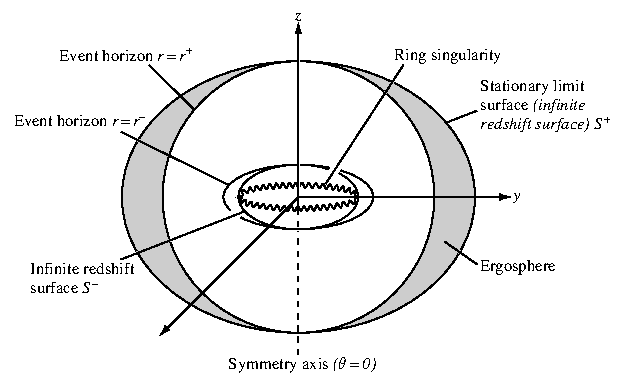
\includegraphics[width=\textwidth]{../images/kerrhole.pdf}
\caption{Diagram showing the structure of a Kerr black hole. It shows the inner and outer ergospheres and event horizons, and the ring singularity in the middle. This kind of black hole has non-zero spin. If the spin was 0 we would have a Schwarzschild black hole instead.
(Figure 13.3 from \cite{grintro})}
\label{fig:KerrHole}
\end{figure}

%TODO

%Kahdenlaista frame draggingia Lense-Thirring efekti pyörivillä

%mainitse Eddingtonin luminositeetti yms jutut? Muuttaa valtavasti massaa energiaksi.

\section{Different types of black holes}

Mass is the only quantity that all black holes have for certain, so it makes sense to categorize them by their mass. They're usually put into three different categories. The reason for this kind of distinction is that the different mass black holes are found in very different kinds of environments and have varying formation methods.%TODO vähennä different käyttöä
The mass limits for the categories aren't exact, but typically stellar mass black holes (SBH) are below $10^2 \ M_\odot$, intermediate mass black holes (IMBH) are between $10^2$ and $10^5 \ M_\odot$, and supermassive black holes (SMBH) are above $10^5 \ M_\odot$.

%kerro eri kohissa et miten voi havaita, mitä eri ilmiöitä nää ehkä synnyttää
%kerro miten syntyvät, massarajoja, tähden kokonaismassa on eri kuin ytimen massa, joka kertoo voiko syntyä musta aukko

\subsection{Stellar mass black holes}

Stellar mass black holes are born from collapsing stars. During their active life, stars stay in equilibrium due to the gravitational pull of the matter making up the star, and the outward pressure caused by the nuclear reactions in the star's core. At the end of the star's lifespan, as its reserves of hydrogen run out, it will start using helium as a new fuel for fusion, and when helium runs out, even heavier elements. For massive enough stars this continues until the star reaches elements such as iron and nickel. Iron has one of the highest binding energies of all the elements, meaning that lighter elements release energy through fusion, but reactions producing heavier elements require additional energy. The star cannot fuse any more matter in its core, and thus the supporting pressure drops, causing the star to implode under its own gravity. Iron being the final product in stars causes what is known as the iron peak in the abundance of chemical elements. Iron is one of the most common metals in the universe, as seen in figure \ref{fig:IronPeak}.

What happens next depends on the mass of the star. For the star to be able to reach this stage, it needs to be over around 8 solar masses. Otherwise it will blow off its atmosphere, leaving behind a white dwarf. In more massive stars, the iron core will exceed the Chandrasekhar limit of around 1.4 solar masses, which describes the upper limit for the mass of a stable white dwarf. Stars above this 8 solar mass threshold but below around 20 solar masses explode in supernovae and leave behind neutron stars. If the initial mass of the star is even higher than that, the supernova remnant is too massive to not collapse into a black hole \citep{woosley:2002}. The actual mass limit is the Tolman–Oppenheimer–Volkoff limit, which gives the upper bound for a cold, non-rotating neutron star, and is about 2.2 solar masses. For stellar remnants more massive than this, the gravitational pull exceeds the neutron pressure keeping the neutron star from collapsing. This also gives a lower limit for the mass of new black holes that form through stellar collapse.

\begin{figure}[h!tb]
\centering
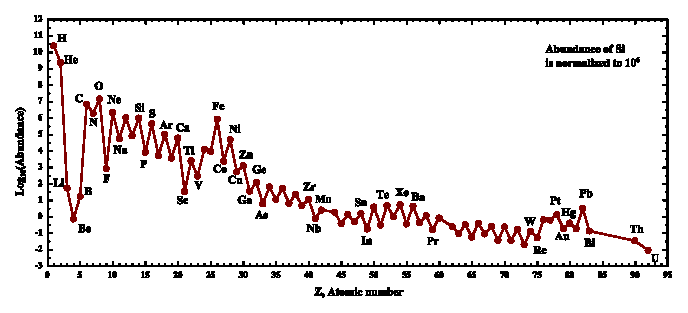
\includegraphics[width=\textwidth]{../images/SolarSystemAbundances.pdf}
\caption{Diagram illustrating the abundancies of different elements in our solar system. Iron has one of the highest binding energies, causing it to be very abundant in the universe thanks to its production in stars before they explode.
(\copyright \ User:MHz\textasciigrave as / Wikimedia Commons / CC-BY-SA-3.0)}
\label{fig:IronPeak}
\end{figure}

One way stellar mass black holes have been observed is in X-ray binaries. These kinds of binaries were discovered through the detection of highly energetic X-ray sources, having luminosities with the same magnitude as the Eddington luminosity. This combined with their low timescale variability (down to milliseconds) lent support for a model where the X-rays are produced by matter from a star accreting onto a compact object. The mass of the compact object $M_x$ can be estimated by measuring the orbital period $P$, radial velocity amplitude $K$, and the mass of the companion star $M_c$, and the inclination angle $i$. These are used in the mass function equation 
\begin{equation}
f(M_x) = \frac{K^3 P}{2 \pi G} = \frac{M_x^3 \mathrm{sin}^3 i}{(M_x + M_c)^2}
\end{equation}
which tells the lower limit for $M_x$ \citep{casares:2007}. The key factor in the equation is $M_c$ which can have a lot of uncertainty. The reason that the mass of the central object is interesting is that both neutron stars and black holes can cause this kind of radiation. But if the mass can be measured to be high above the aforementioned Tolman–Oppenheimer–Volkoff limit, other objects than black holes can be quite safely ruled out.

%puhu muista tavoista havaita, värihommaa?
%neutronitähdissä voi olla flareja

%fuusiokartta, raudasta ei pääse eteenpäin, iron peak

%observable in x-ray compact binary systems

\subsection{Intermediate mass black holes}

Intermediate mass black holes are much more elusive compared to both their more massive and lighter companions. We have very few good candidates and their formation is not fully understood.

One way for these kinds of black holes to form could be through massive Population III stars. These stars formed early in the universe and thus they had very low metallicities. This allows them to grow very large, and the mass of Pop III stars can exceed 200 solar masses. These stars can also retain their mass as they exhibit weaker stellar winds compared to more metal-rich stars. When these stars collapse in a similar manner to lower mass stars, they could then form black holes with masses of several hundred $M_\odot$. Another prediction for their formation is through multiple collisions of lower mass compact objects in regions with dense stellar populations, such a stellar clusters \citep{koliopanos:2017}.

\subsection{Supermassive black holes}


\section{Newtonian dynamics}

%perusjuttua newtonin dynamiikasta

\section{Regularization}

Because of the $1/r^2$ term in the Newtonian equations of motion, the N-body problem becomes singular when the distance between two objects approaches zero. It is because of these singularities that the analysis of the N-body problem becomes very arduous when collisions or close approaches occur. That is why it would be desirable to get rid of these singularities on the equation of motion. This is achieved with regularization, which just means finding a different set of equations that do not exhibit this singularity when $r$ approaches zero.

Usually this comes with the cost of having a higher number of variables to keep track of. But regularization shows great advantages in the time-step sizes needed for accurate integration, and the amount of time-steps needed for integrating close encounters is much smaller. 

\section{Post-Newtonian dynamics}

While Newtonian dynamics is a perfectly valid approximation in everyday life, it stops giving correct results when more massive or faster moving objects are concerned, and instead we need to use general relativity (GR). %TODO Selitä geeärrää?
Doing fully general relativistic simulations is very computationally intensive however, so more wieldy methods are required for large scale simulations. This is where post-Newtonian (PN) expansions come in. Post-Newtonian expansions in general relativity are used for finding an approximate solution of the Einstein field equations for the metric tensor. %TODO selitä noi lisäks
Einstein field equations are the set of 10 equations in Albert Einstein's general theory of relativity that describe the fundamental interaction of gravitation as a result of spacetime being curved by mass and energy.
In other words, the post-Newtonian theory is an approximate version of general relativity that applies when the gravitational field is relatively weak, and the motion of the matter is slow. The theory successfully describes the gravitational field of our solar system, but it can also be applied to situations involving compact bodies with strong internal gravity, provided that the mutual gravity between bodies is weak enough.

The post-Newtonian theory is derived from the Landau-Lifshitz formulation of the Einstein field equations. The equations can be written as 
\begin{equation}
\partial_{\mu \nu} H^{\alpha \mu \beta \nu} = \frac{16 \pi G}{c^4}(-g)(T^{\alpha \beta} + t^{\alpha \beta}_{LL}) \ ,
\end{equation}
where $H^{\alpha \mu \beta \nu} \equiv \mathfrak{g}^{\alpha \beta} \mathfrak{g}^{\mu \nu} - \mathfrak{g}^{\alpha \mu} \mathfrak{g}^{\beta \mu}$ is a tensor density which possesses the same symmetries as the Riemann tensor. In the Landau-Lifshitz formulation the main variables are not the components of the metric tensor $g_{\alpha \beta}$, but those of the gothic inverse metric $\mathfrak{g}^{\alpha \beta} \equiv \sqrt{-g} g^{\alpha \beta}$, where $g^{\alpha \beta}$ is the inverse metric, and $g$ the metric determinant. $T^{\alpha \beta}$ is the energy-momentum tensor of the matter source term, and the Landau-Lifshitz pseudotensor $(-g) t^{\alpha \beta}_{LL} \sim \partial \mathfrak{g} \cdot \partial \mathfrak{g}$ can be interpreted as an energy-momentum (pseudo)tensor for the gravitational field.

The antisymmetry of $H^{\alpha \mu \beta \nu}$ implies the conservation equation
\begin{equation}
\partial_\beta \left[ (-g)(T^{\alpha \beta} + t^{\alpha \beta}_{LL}) \right] = 0 \ ,
\end{equation}
which is formally equivalent to $\nabla_\beta T^{\alpha \beta} = 0$, where $\nabla_\beta$ is the covariant derivative operator. The conservation equation allows for the formulation of global conservation laws, for example for energy, linear momentum, and angular momentum. We then introduce the gravitational potentials $h^{\alpha \beta} = \eta^{\alpha \beta} - \mathfrak{g}^{\alpha \beta}$, where $\eta^{\alpha \beta} = diag(-,+,+,+)$ is the Minkowski metric expressed in Lorentzian coordinates, and impose the harmonic coordinate gauge condition $\partial_\beta h^{\alpha \beta} = 0$.

The field equations become a wave equation in flat spacetime
\begin{equation} \label{equ:waveeq}
\square h^{\alpha \beta} = -\frac{16 \pi G}{c^4} \tau^{\alpha \beta} \ ,
\end{equation}
where $\square = -\frac{1}{c^2} \frac{\partial^2}{\partial t^2} + \frac{\partial^2}{\partial x^2} + \frac{\partial^2}{\partial y^2} + \frac{\partial^2}{\partial z^2}$ is the flat spacetime d'Alembert operator, and $\tau^{\alpha \beta} = (-g)(T^{\alpha \beta} + t^{\alpha \beta}_{LL} + t^{\alpha \beta}_H)$ is defined as the effective energy-momentum pseudotensor, composed of a matter contribution, the Landau-Lifshitz contribution, and the harmonic gauge contribution $t^{\alpha \beta}_H \sim \partial h \cdot \partial h + h \partial^2 h$. The conversation equation now reads $\partial_\beta \tau^{\alpha \beta} = 0$.

So far no approximations have been made, and the wave equation combined with the harmonic gauge condition and conservation equation is an exact formulation of the Einstein field equations. The wave equation determines the potential $h^{\alpha \beta}$ for a given distribution of matter. The behaviour of the matter is determined by the conservation equation/gauge condition.

The wave equation can be integrated without enforcing the conservation equation, and this is known as the relaxed Einstein field equations. The integration is achieved by iteration. Assuming that $h^{\alpha \beta}_n$ is known, $h^{\alpha \beta}_{n+1}$ is obtained by solving
\begin{equation}
\square h^{\alpha \beta}_{n+1} = -\frac{16 \pi G}{c^4} \tau^{\alpha \beta}[h_n] \ .
\end{equation}
The iterations are started with $h^{\alpha \beta}_0 = 0$, and stopped when the desired accuracy is obtained. In principle, the truncation is the only source of approximation. The procedure produces a formal expansion of $h^{\alpha \beta}$ in powers of G. This is known as the post-Minkowskian expansion of the gravitational field. After iterations have been done up to the desired accuracy, we can again impose the gauge condition to get a proper metric.

The difference between post-Minkowskian and post-Newtonian expansion is that in post-Newtonian approximation we assume a slow-motion condition, i.e. all speeds within the matter
distribution (such as the speed of sound within a body, or the speed of the body as a whole)
are small compared with the speed of light. In astrophysical situations the assumption of slow speeds is accurate in the vast majority of cases, since the virial theorem implies that $U \sim v^2$ for any gravitationally bound system; weak fields are naturally accompanied by slow motion.



The approximations are expanded in small parameters which express orders of deviations from Newton's laws of gravity. A correction of order $(v/c)^n$ to a Newtonian expression is said to be of $\mathrm{PN}(n/2)$ order.

The first use of a PN expansion (to first order) was made by Einstein in calculating the perihelion precession of Mercury's orbit.
Mercury's perihelion precesses (rotates) around the sun. This is mainly due to perturbations caused by the presence of the other planets. Another much less significant factor is the oblateness of the sun. In the 1800s it was noticed that the orbit deviates from the precession predicted by these Newtonian effects by about 43 arc seconds per a tropical century.

Several different reasons for this deviation were proposed, and perhaps the most prevalent of these was Vulcan. Vulcan is a small hypothetical planet that was supposed to orbit the sun inside the orbit of Mercury. The perturbations caused by this planet could have explained the anomalous precession of Mercury. The existence of the planet was hypothesized by the French mathematician Urbain Le Verrier, who also predicted the existence and position of Neptune with only mathematics. While many people claimed to have observed the planet, its supposed orbit was so close to the sun that this was extremely challenging to verify.

There were attempts to confirm the existence of the planet, but in 1915 the hypothetical planet was quite firmly put to rest when Einstein explained the anomalous precession through his theory of relativity. The reason why the same extra precession that affects all of the planets had been observed only with Mercury is that the magnitude of the differences from simple Newtonian theory diminishes rapidly as one gets farther from the Sun. Mercury's fairly eccentric orbit also makes it much easier to detect the perihelion shift than is the case for the nearly circular orbits of Venus and Earth.
This was the first case of solving the general relativistic two-body problem, which is the most common use of the PN expansion nowadays. %TODO Lisää hommaa, toimii myös aurinkokunnassa, referenssejä Vulkanukseen wikipediasta

%Hyvää matskua: gravity postminkowskian implementation sivu 10, gravity postnewtonian fundamental heti alku, common reader 3.2

In the case of a two-body system, the post-Newtonian corrections give rise to a perturbed Keplerian orbit. The only secular effect on the orbit is the pericenter advance.
PN1 terms are the ones responsible for the advance of the pericenter of an eccentric orbit, given by $\dot{\omega} = 6 \pi f_\mathrm{b} m/a (1-e^2)$, where $a$ and $e$ are the semimajor axis and eccentricity of the orbit, and $f_\mathrm{b}$ is the orbital frequency, given by Kepler's third law $2 \pi f_\mathrm{b} = (m/a^3)^{1/2}$ \citep{will:2006}. 

The intrinsic angular momentum (spin) of a body is also a source of gravity that affects the metric and body motions. The spin causes precession in the ascending node. %TODO lisää kaavaa, gravity kalvoista

There are some systems that cannot be properly described by post-Newtonian approximation because of their extreme conditions. Some examples of such systems include the final phases of a compact object merger, the cores of supernovae, and the structure of rapidly rotating neutron stars. These must be analysed using different methods, for example the full solution of Einstein's equations via numerical methods \citep{will:2006}. 

\section{Black holes in galaxy mergers}

\section{Black hole mergers}
\subsection{Dynamical friction}
\subsection{Three body scattering}
\subsection{Gravitational waves}

\chapter{AR-CHAIN}
\section{AR-CHAIN overview}

The code uses post-Newtonian corrections to take into account and approximate the relativistic effects near the black hole particles. The corrections are represented by additional terms in the relative accelerations of the two bodies, so that
\begin{equation}
\boldsymbol{a}_\mathrm{2-body} = \boldsymbol{a}_\mathrm{Newtonian} + \sum_{k=2}^7 c^{-k} \boldsymbol{a}_\mathrm{(k/2)PN} + \boldsymbol{a}_S \ ,
\end{equation}
where $\boldsymbol{a}_\mathrm{Newtonian}$ is the usual Newtonian two-body acceleration, $c$ is the speed of light, $\boldsymbol{a}_\mathrm{xPN}$ is the PN correction of order $x$, and $\boldsymbol{a}_S$ indicates PN terms depending on the spins of the particles. PN corrections up to order PN3.5 are included in the code.

For spinning bodies, additional PN corrections are required. The PN contribution to the equations of motion for the spins is given by
\begin{equation}
\boldsymbol{\dot{S}}_i = \boldsymbol{S}_{\mathrm{PN},i} \times \boldsymbol{S}_i \ ,
\end{equation}
where $\boldsymbol{S}_i$ is the spin angular momentum of the particle $i$ and $\boldsymbol{S}_{\mathrm{PN},i}$ gives the effect of the spin-orbit, spin-spin, and quadrupole-monopole interactions. %TODO Selitä näitä pls

These two-body PN corrections are only used when at least one of the bodies is a black hole, since for other particles they're not of any significance. Only when a black hole is involved are the velocities and masses large enough to require relativistic treatment.

\section{Bulirsch–Stoer algorithm}
\section{Time-transformed leapfrog}
\section{Collisions}

\chapter{KETJU}
\section{KETJU overview}
\section{}
\section{}

\chapter{AR-CHAIN results}
\section{OJ287}

These following runs all had similar initial conditions, apart from the magnitude of the spin. The initial values for the orbital elements were those measured by Valtonen \& Mikkola (cite), with the semimajor axis of the binary being around 11350 AU, the eccentricity being 0.6, and spin being 0.28. Simulations were also run with a spin of 0 and a spin three times the original. The direction of the spin was towards the positive z-axis of the system. The inclination of the orbit was 45 degrees in the xz-plane. So the spin was inclined 45 degrees to the initial orbit. The initial timestep in the simulations was 0.01 gadget times, and the interval for writing the data in a file was 1 gadget time. 

The orbital elements precessed, so average values were used to make smoother and clearer graphs. 

The eccentricity of the orbit goes down as the orbit circularizes due to the GW emissions.

The PN2.5 term is responsible for the GW emissions.

The spin caused the orbit to twist. This can be seen clearly in images \ref{fig:spin0Orbits} and \ref{fig:spinNormalOrbits}. If there was no spin, the orbit stayed neatly in the original plane, but with spin the orbit started turning.

One should keep in mind that this model is very simplistic. There are only the two black holes, and no other stars to interact with, and no accretion disks, which are thought to play a relatively large role in the life of the system.

\begin{figure}[h!tb]
\centering
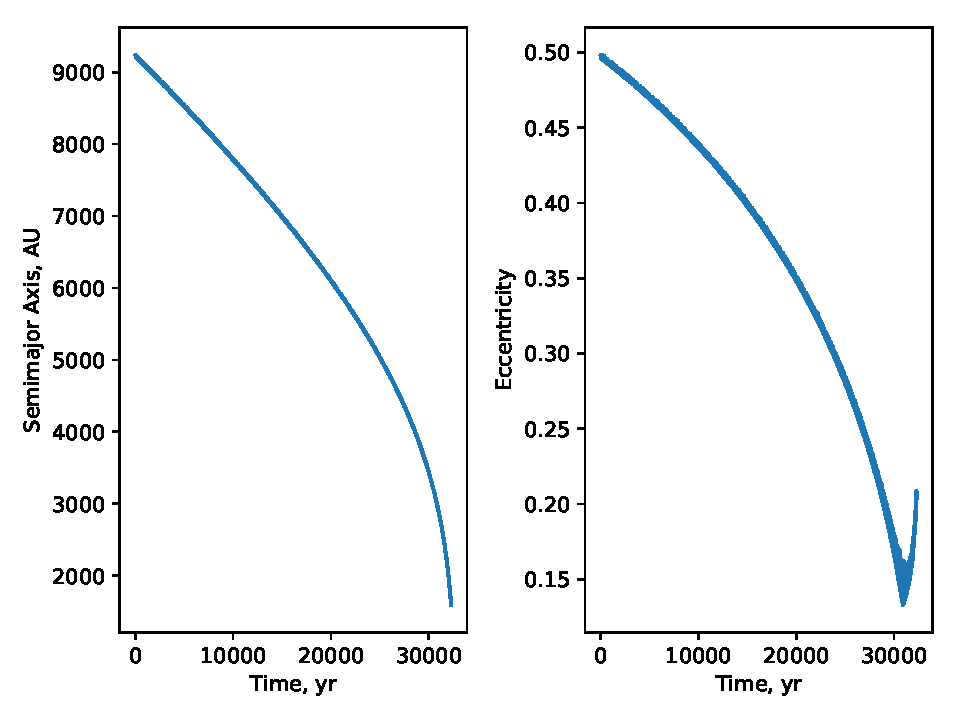
\includegraphics[width=\textwidth]{../images/spinNormal.pdf}
\caption{The development of the semimajor axis and eccentricity of the smaller of the two black holes in the binary, with it having a spin of 0.28. The merging happened at around 206800 gadget time, corresponding to 32300 years.}
\label{fig:spinNormal}
\end{figure}

\begin{figure}[h!tb]
\centering
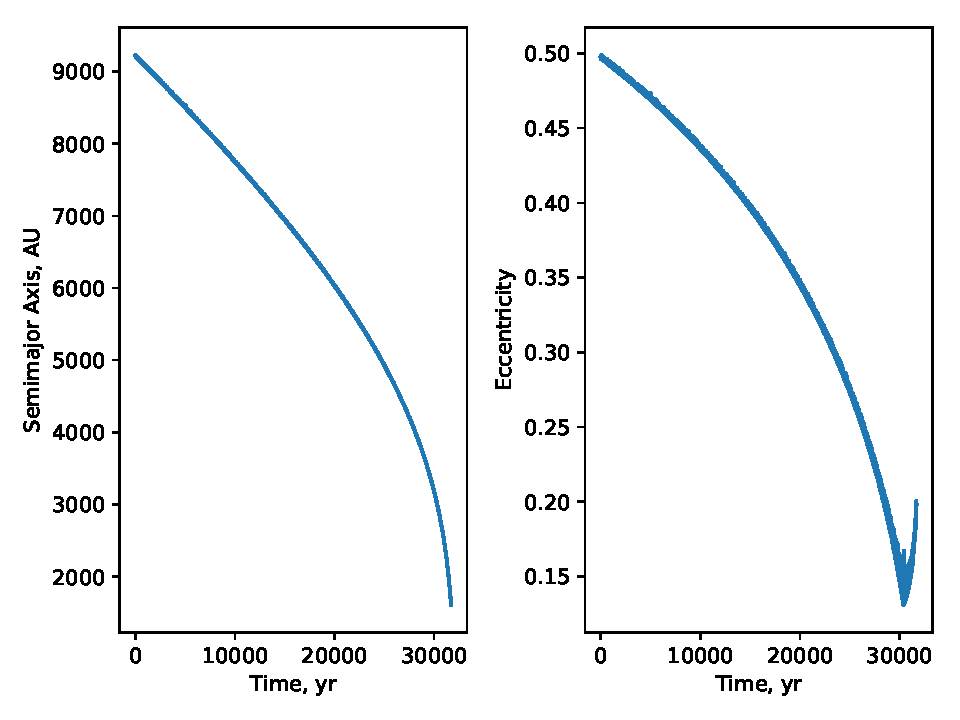
\includegraphics[width=\textwidth]{../images/spin0.pdf}
\caption{The development of the semimajor axis and eccentricity of the smaller of the two black holes in the binary, with it having no spin at all. The merging happened at around 202300 gadget time, corresponding to 31700 years.}
\label{fig:spin0}
\end{figure}

\begin{figure}[h!tb]
\centering
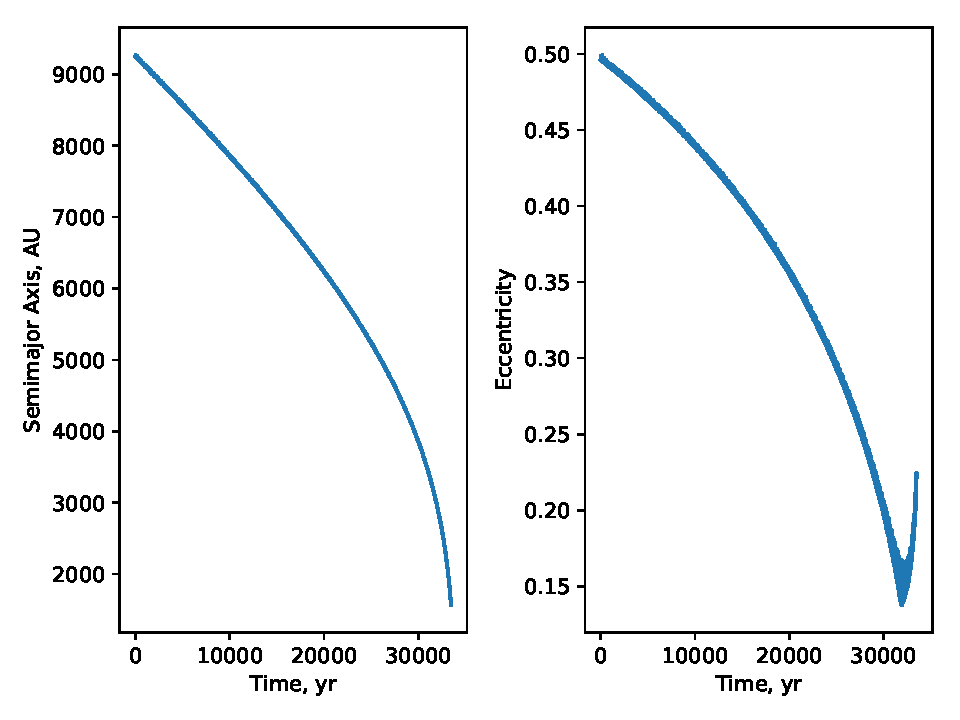
\includegraphics[width=\textwidth]{../images/spin3.pdf}
\caption{The development of the semimajor axis and eccentricity of the smaller of the two black holes in the binary, with it having a spin of 0.84, three times the real value. The merging happened at around 214400 gadget time, corresponding to 33500 years.}
\label{fig:spin3}
\end{figure}

\begin{figure}[h!tb]
\centering
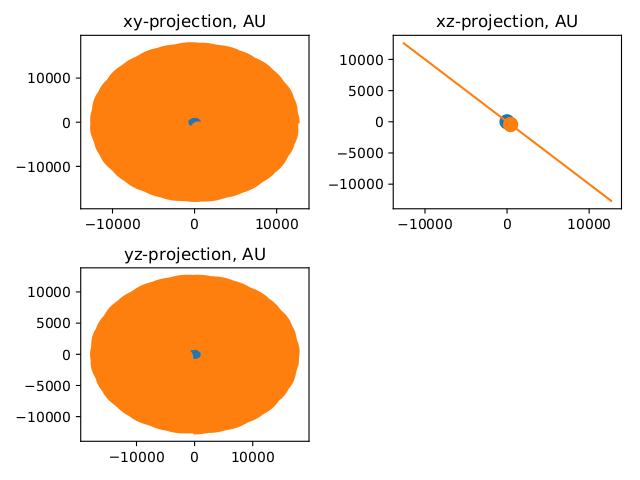
\includegraphics[width=\textwidth]{../images/spin0Orbits.png}
\caption{Plot of the the orbits of the binary if there is no spin. The orbiting member doesn't leave the original plane it was in.}
\label{fig:spin0Orbits}
\end{figure}

\begin{figure}[h!tb]
\centering
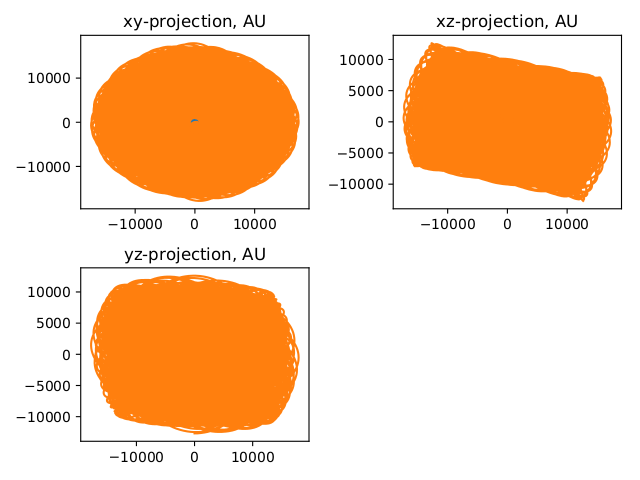
\includegraphics[width=\textwidth]{../images/spinNormalOrbits.png}
\caption{Plot of the the orbits of the binary with the measured spin.}
\label{fig:spinNormalOrbits}
\end{figure}

\begin{figure}[h!tb]
\centering
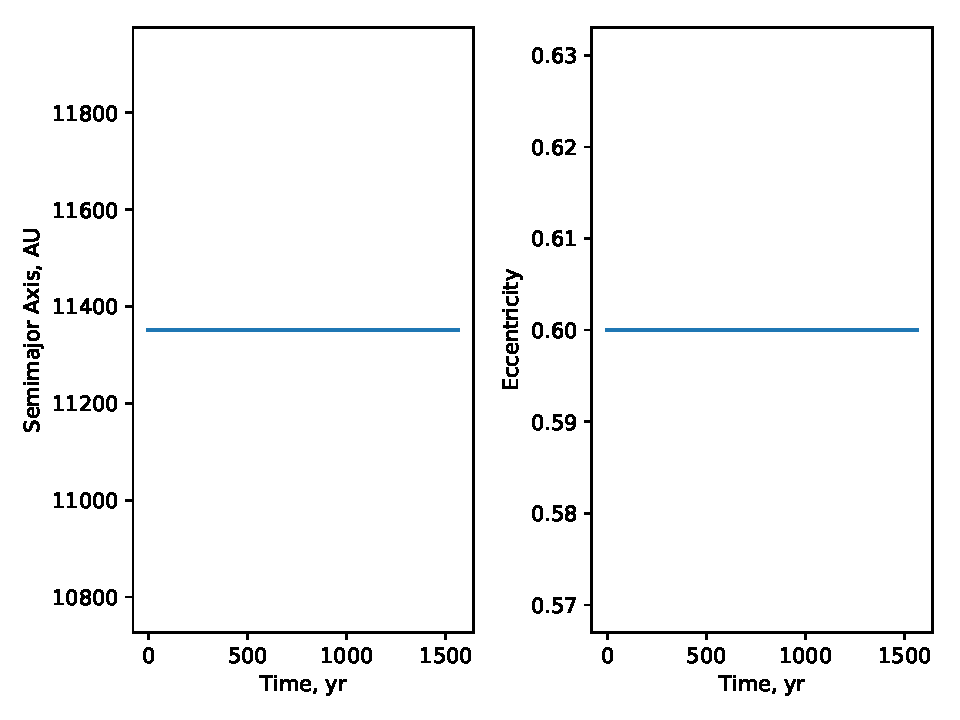
\includegraphics[width=\textwidth]{../images/noPN.pdf}
\caption{The development of the semimajor axis and eccentricity of the smaller of the two black holes in the binary, if the post-Newtonian terms aren't factored in. The simulation was run for slightly over 1500 years. Since the PN terms were not taken into account the orbit didn't actually decay, just as expected. The results themselves aren't very interesting, but it shows that the corrections are indeed needed for realistic results.}
\label{fig:noPN}
\end{figure}

\subsection{Estimated time of merging}
\subsection{Differences from reality}
\section{Effects of spin}

\chapter{KETJU results}
\section{}

\chapter{Conclusions}

% STEP 5:
% Uncomment the following lines and set your .bib file and desired bibliography style
% to make a bibliography with BibTeX.
% Alternatively you can use the thebibliography environment if you want to add all
% references by hand.

\clearpage
\addcontentsline{toc}{chapter}{Bibliography} % This lines adds the bibliography to the ToC
\bibliographystyle{plainnat}
\small
\bibliography{lahteet}


\end{document}

